\lab{Iterative Solvers}{Iterative Solvers}
\label{lab:iter_methods}

\objective{
Many real-world problems of the form $A\x =\b$ have tens of thousands of parameters.
Solving such systems with Gaussian elimination or matrix factorizations could require trillions of floating point operations (FLOPs), which is of course infeasible.
Solutions of large systems must therefore be approximated iteratively.
In this lab, we implement three popular iterative methods for solving large systems: Jacobi, Gauss-Seidel, and Successive Over-Relaxation.}

% Though finding an exact solution is either very time intensive or unstable, iterative methods give a sufficiently close approximations and take much less time.

Iterative methods are often useful to solve large systems of equations.
In this lab, let $\x^{(k)}$ denote the $k$th iteration of the iterative method for solving the problem $A\x=\b$ for $\x$.
Furthermore, let $x_{i}$ be the $i$th component of $\x$ so that $x_{i}^{(k)}$ is the $i$th component of $\x$ in the $k$th iteration.
Like other iterative methods, there are two stopping parameters: a very small $\epsilon > 0$ and an integer $N\in\mathbb{N}$.
Iterations continue until either
\begin{equation} % Stopping Criteria.
\|\x^{(k-1)}-\x^{(k)}\| < \epsilon
\qquad \text{or} \qquad
k > N.
\label{eq:itersolve-stopping-criteria}
\end{equation}

\section*{The Jacobi Method} % ================================================

The \emph{Jacobi Method} is a simple but powerful method used for solving certain kinds of large linear systems.
The main idea is simple: solve for each variable in terms of the others, then use the previous values to update each approximation.
As a (very small) example, consider the $3 \times 3$
\begin{align*}
\begin{array}{ccccccr}
  2x_1 &   &      & - & x_3  & = & 3,  \\
  -x_1 & + & 3x_2 & + & 2x_3 & = & 3,  \\
       & + & x_2  & + & 3x_3 & = & -1. \\
\end{array}
\end{align*}

Solving the first equation for $x_1$, the second for $x_2$, and the third for $x_3$ yields
\begin{align*}
\begin{array}{ccc}
    x_1 & = & \frac{1}{2}(3 + x_3), \\
    x_2 & = & \frac{1}{3}(3 + x_1 - 2x_3), \\
    x_3 & = & \frac{1}{3}(-1 - x_2).
\end{array}
\end{align*}

Now begin with an initial guess $\x^{(0)} = [x^{(0)}_1, x^{(0)}_2, x^{(0)}_3]\trp = [0,0,0]\trp$.
To compute the first approximation $\x^{(1)}$, use the entries of $\x^{(0)}$ as the variables on the right side of the previous equations:
\begin{align*}
\begin{array}{ccccccr}
    x^{(1)}_1 & = & \frac{1}{2}(3 + x^{(0)}_3) & = & \frac{1}{2} (3 + 0) & = & \frac{3}{2}, \\
    x^{(1)}_2 & = & \frac{1}{3}(3 + x^{(0)}_1 - 2x^{(0)}_3) & = & \frac{1}{3} (3 + 0 - 0) & = & 1, \\
    x^{(1)}_3 & = & \frac{1}{3}(-1 - x^{(0)}_2) & = & \frac{1}{3} (-1 - 0) & = & -\frac{1}{3}. \\
\end{array}
\end{align*}

Thus $\mathbf{x}^{(1)} = [\frac{3}{2}, 1, -\frac{1}{3}]\trp$.
Computing $\mathbf{x}^{(2)}$ is similar:
\begin{align*}
\begin{array}{ccccccc}
x^{(2)}_1 & = & \frac{1}{2} ( 3 + x^{(1)}_3)  & = & \frac{1}{2} (3 - \frac{1}{3})     & = & \frac{4}{3}, \\
x^{(2)}_2 & = & \frac{1}{3} ( 3 + x^{(1)}_1 - 2x^{(1)}_3) & = & \frac{1}{3} (3 + \frac{3}{2} + \frac{2}{3}) & = &  \frac{31}{18}, \\
x^{(2)}_3 & = & \frac{1}{3} ( -1 - x^{(1)}_2)       & = & \frac{1}{3} (-1 - 1)    & = & -\frac{2}{3}. \\
\end{array}
\end{align*}

The process is repeated until at least one of the two stopping criteria in (\ref{eq:itersolve-stopping-criteria}) is met.
For this particular problem, convergence to 8 decimal places ($\epsilon = 10^{-8}$) is reached in 29 iterations.

\begin{center}
\begin{tabular}{c|ccc}
    & $x^{(k)}_1$ & $x^{(k)}_2$ & $x^{(k)}_3$ \\
    \hline
    $\x^{(0)}$ & $0$ & $0$ & $0$ \\
    %\hline
    $\x^{(1)}$ & $1.5$ & $1$ & $-0.33333333$ \\
    %\hline
    $\x^{(2)}$  & $1.33333333$ & $1.72222222$ & $-0.6666666$7 \\
    $\x^{(3)}$  & $1.16666667$ & $1.88888889$ & $-0.9074074$1 \\
    $\x^{(4)}$  & $1.04629630$ & $1.99382716$ & $-0.9629629$6 \\
    \vdots      & \vdots       & \vdots       & \vdots      \\
    $\x^{(28)}$ & $0.99999999$ & $2.00000001$ & $-0.9999999$9 \\
    $\x^{(29)}$ & $1$          & $2$          & $-1$          \\
\end{tabular}
\end{center}

\subsection*{Matrix Representation} % -----------------------------------------

The iterative steps performed above can be expressed in matrix form.
First, decompose $A$ into its diagonal entries, its entries below the diagonal, and its entries above the diagonal, as $A = D + L + U$.
\begin{align*}
\begin{array}{ccccc}
    \left[\begin{array}{cccc}
        a_{11} & 0 & \ldots & 0 \\
        0 & a_{22} & \ldots & 0 \\
        \vdots & \vdots & \ddots & \vdots \\
        0 & 0 & \ldots & a_{nn} \\
    \end{array}\right]
    & &
    \left[\begin{array}{cccc}
    0 & 0 & \ldots & 0 \\
    a_{21} &  0 & \ldots & 0\\
     \vdots & \ddots & \ddots & \vdots \\
    a_{n1} & \ldots & a_{n,n-1} & 0 \\
    \end{array}\right]
    & &
    \left[\begin{array}{cccc}
    0 & a_{12} & \ldots & a_{1n} \\
    0 & 0 & \ddots & \vdots \\
     \vdots & \vdots & \ddots & a_{n-1,n} \\
    0 & 0 & \ldots & 0 \\
    \end{array}\right]
    \\D & & L & & U
\end{array}
\end{align*}

With this decomposition, $\x$ can be expressed in the following way.
\begin{align*}
A\x &= \b\\
(D + L + U)\x &= \b\\
D\x &= -(L+U)\x + \b\\
\x &= D^{-1}(-(L+U)\x + \b)
\end{align*}

Now using $\x^{(k)}$ as the variables on the right side of the equation to produce $\x^{(k+1)}$ on the left, and noting that $L+U=A-D$, we have the following.
\begin{align}
\nonumber \x^{(k+1)} &= D^{-1}(-(A-D)\x^{(k)} + \b) \\
\nonumber &= D^{-1}(D\x^{(k)} - A\x^{(k)}  + \b)\\
&= \x^{(k)} + D^{-1}(\b - A\x^{(k)})
\label{eq:jacobi-method}
\end{align}

There is a potential problem with (\ref{eq:jacobi-method}): calculating a matrix inverse is the cardinal sin of numerical linear algebra, yet the equation contains $D^{-1}$.
However, since $D$ is a diagonal matrix, $D^{-1}$ is also diagonal, and is easy to compute.

\[
D^{-1} =
\left[\begin{array}{cccc}
    \frac{1}{a_{11}} & 0                & \ldots & 0      \\
    0                & \frac{1}{a_{22}} & \ldots & 0      \\
    \vdots           & \vdots           & \ddots & \vdots \\
    0                & 0                & \ldots & \frac{1}{a_{nn}}
\end{array}\right]
\]
Because of this, the Jacobi method requires that $A$ have nonzero diagonal entries.

The diagonal $D$ can be represented by the 1-dimensional array $\mathbf{d}$ of the diagonal entries. %(instead of as a 2-dimensional array).
Then the matrix multiplication $D\x$ is equivalent to the component-wise vector multiplication $\mathbf{d}*\x = \x*\mathbf{d}$.
Likewise, the matrix multiplication $D^{-1}\x$ is equivalent to the component-wise ``vector division'' $\x/\mathbf{d}$.

\begin{comment}% This didn't seem super useful so I took it out.
\begin{lstlisting}
>>> import numpy as np

>>> D = np.array([[2,0],[0,16]])    # Let D be a diagonal matrix.
>>> d = np.diag(D)                  # Extract the diagonal as a 1-D array.
>>> x = np.random.random(2)
>>> np.allclose(D.dot(x), d*x)
<<True>>
\end{lstlisting}
\end{comment}

\begin{comment} % Jacobi algorithm box. Probably unnecessary.
\begin{algorithm}[H]
\begin{algorithmic}[1]
\Procedure{Jacobi Method}{$A$, $\b$, $\epsilon$, $N$}
    \State $m, n \gets \shape{A}$
        \Comment{Store the dimensions of $A$.}
    \State $\mathbf{d} \gets$ diag($A$)
        \Comment{Get the diagonal entries of $A$ with \li{np.diag()}.}
    \State $\x^{(0)} \gets \zeros{n}$
        \Comment{An array of $n$ zeros.}
    \For{$k=0 \ldots N-1$}
        \State $\x^{(k+1)} \gets (\b - A\x^{(k)} + \mathbf{d}*\x^{(k)})/\mathbf{d}$
        \If{$\|\mathbf{x}^{(k-1)} - \mathbf{x}^{(k)}\|_{\infty} < \epsilon$}
            \State \pseudoli{break}
        \EndIf
    \EndFor
    \State \pseudoli{return} $\x^{(k)}$
\EndProcedure
\end{algorithmic}
\caption{}
\label{alg:jacobi-method}
\end{algorithm}
\end{comment}

\begin{problem} % Implement the Jacobi Method.
Write a function that accepts a matrix $A$, a vector $\b$, a convergence tolerance \li{tol} defaulting to $10^{-8}$, and a maximum number of iterations \li{maxiter} defaulting to $100$.
Implement the Jacobi method using (\ref{eq:jacobi-method}), returning the approximate solution to the equation $A\x = \b$.

Run the iteration until $\|\mathbf{x}^{(k-1)} - \mathbf{x}^{(k)}\|_{\infty} <$ \li{tol}, and only iterate at most \li{maxiter} times.
Avoid using \li{la.inv()} to calculate $D^{-1}$, but use \li{la.norm()} to calculate the vector $\infty$-norm.

% \begin{lstlisting}
% >>> from scipy import linalg as la
%
% >>> x = np.random.random(10)
% >>> la.norm(x, <<ord>>=np.inf)          # Use la.norm() for ||x||.
% 0.74623726404168045
% >>> np.<<max>>(np.<<abs>>(x))               # The equivalent in NumPy for ||x||.
% 0.74623726404168045
% \end{lstlisting}

Your function should be robust enough to accept systems of any size.
To test your function, generate a random $\b$ with \li{np.random.random()} and use the following function to generate an $n\times n$ matrix $A$ for which the Jacobi method is guaranteed to converge.
Run the iteration, then check that $A\x^{(k)}$ and $\b$ are close using \li{np.allclose()}.

\begin{lstlisting}
def diag_dom(n, num_entries=None):
    """Generate a strictly diagonally dominant (n, n) matrix.
    Parameters:
        n (int): The dimension of the system.
        num_entries (int): The number of nonzero values.
            Defaults to n^(3/2)-n.
    Returns:
        A ((n,n) ndarray): A (n, n) strictly diagonally dominant matrix.
    """
    if num_entries is None:
        num_entries = int(n**1.5) - n
    A = np.zeros((n,n))
    rows = np.random.choice(np.arange(0,n), size=num_entries)
    cols = np.random.choice(np.arange(0,n), size=num_entries)
    data = np.random.randint(-4, 4, size=num_entries)
    for i in range(num_entries):
        A[rows[i], cols[i]] = data[i]
    for i in range(n):
        A[i,i] = np.<<sum>>(np.<<abs>>(A[i])) + 1
    return A
\end{lstlisting}

Also test your function on random $n \times n$ matrices.
If the iteration is non-convergent, the successive approximations will have increasingly large entries.

\label{prob:jacobi}
\end{problem}

\subsection*{Convergence} % ---------------------------------------------------

Most iterative methods only converge under certain conditions.
For the Jacobi method, convergence mostly depends on the nature of the matrix $A$.
If the entries $a_{ij}$ of $A$ satisfy the property
\[
|a_{ii}| > \sum_{j \neq i} |a_{ij}|\quad \text{for all}\quad i = 1,2,\ldots,n,
\]
then $A$ is called \emph{strictly diagonally dominant} (\li{diag_dom()} in Problem \ref{prob:jacobi} generates a strictly diagonally dominant $n\times n$ matrix).
If this is the case,\footnote{Although this seems like a strong requirement, most real-world linear systems can be represented by strictly diagonally dominant matrices.} then the Jacobi method always converges, regardless of the initial guess $\x_0$.
This is a very different convergence result than many other iterative methods such as Newton's method where convergence is highly sensitive to the initial guess.

There are a few ways to determine whether or not an iterative method is converging.
For example, since the approximation $\x^{(k)}$ should satisfy $A\x^{(k)} \approx \b$, the normed difference $\|A\x^{(k)} - \b\|_\infty$ should be small.
This value is called the \emph{absolute error} of the approximation.
If the iterative method converges, the absolute error should decrease to $\epsilon$.

\begin{problem}
Modify your Jacobi method function in the following ways.
\begin{enumerate}
    \item Add a keyword argument called \li{plot}, defaulting to \li{False}.
    \item Keep track of the absolute error $\|A\mathbf{x}^{(k)} - \mathbf{b}\|_{\infty}$ of the approximation at each iteration.
    \item If \li{plot} is {True}, produce a lin-log plot (use \li{plt.semilogy()}) of the error against iteration count.
    Remember to still return the approximate solution $\x$.
\end{enumerate}
If the iteration converges, your plot should resemble the following figure.

\begin{figure}[H]
    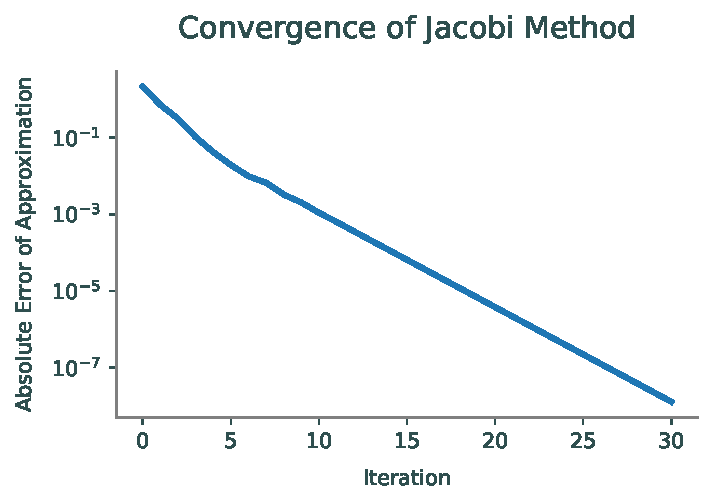
\includegraphics[width=.7\textwidth]{figures/jacobi_convergence.pdf}
\end{figure}

\label{prob:plot-iterative-convergence}
\end{problem}

\section*{The Gauss-Seidel Method} % ==========================================

The \emph{Gauss-Seidel method} is essentially a slight modification of the Jacobi method.
The main difference is that in Gauss-Seidel, new information is used immediately.
As an example, consider again the system from the previous section,
\begin{align*}
\begin{array}{ccccccr}
  2x_1 &   &      & - & x_3  & = & 3,  \\
  -x_1 & + & 3x_2 & + & 2x_3 & = & 3,  \\
       & + & x_2  & + & 3x_3 & = & -1. \\
\end{array}
\end{align*}

As with the Jacobi method, solve for $x_1$ in the first equation, $x_2$ in the second equation, and $x_3$ in the third equation:
\begin{align*}
\begin{array}{ccc}
    x_1 & = & \frac{1}{2}(3 + x_3), \\
    x_2 & = & \frac{1}{3}(3 + x_1 - 2x_3), \\
    x_3 & = & \frac{1}{3}(-1 - x_2).
\end{array}
\end{align*}
Using $\x^{(0)}$ to compute $x^{(1)}_1$ in the first equation as before,
\[x^{(1)}_1 = \frac{1}{2}(3 + x^{(0)}_3) = \frac{1}{2}(3 + 0) = \frac{3}{2}.\]
Now, however, use the updated value of $x^{(1)}_1$ in the calculation of $x^{(1)}_2$:
\[x^{(1)}_2 = \frac{1}{3}(3 + x^{(1)}_1 - 2x^{(0)}_3) = \frac{1}{3}(3 + \frac{3}{2} - 0) = \frac{3}{2}.\]
Likewise, use the updated values of $x^{(1)}_1$ and $x^{(1)}_2$ to calculate $x^{(1)}_3$:
\[x^{(1)}_3 = \frac{1}{3}(-1 - x^{(1)}_2) = \frac{1}{3}(-1 - \frac{3}{2}) = -\frac{5}{6}.\]
This process of using calculated information immediately is called \emph{forward substitution}, and causes the algorithm to (generally) converge much faster.

\begin{center}
\begin{tabular}{c|ccc}
    & $x^{(k)}_1$ & $x^{(k)}_2$ & $x^{(k)}_3$ \\
    \hline
      $x^{(0)}$ & $0$ & $0$ & $0$ \\
      %\hline
      $x^{(1)}$ & $1.5$ & $1.5$ & $-0.83333333$ \\
      %\hline
      $x^{(2)}$ & $1.08333333$ & $1.91666667$ & $-0.97222222$ \\
      $x^{(3)}$ & $1.01388889$ & $1.98611111$ & $-0.99537037$ \\
      $x^{(4)}$ & $1.00231481$ & $1.99768519$ & $-0.99922840$ \\
      \vdots    & \vdots       & \vdots       & \vdots     \\
      $x^{(11)}$ & $1.00000001$ & $1.99999999$ & $-1$ \\
      $x^{(12)}$ & $1$ & $2$ & $-1$ \\
\end{tabular}
\end{center}
Notice that Gauss-Seidel converges in less than half as many iterations as Jacobi does for this system.

\subsection*{Implementation} % ------------------------------------------------

% This matches the book (Ch. 13), but it may be confusing to the students here.
% We begin by solving for $\x$ in a slightly different way.
% \begin{align}
% \nonumber A\x &= \b\\
% \nonumber (D + L + U)\x &= \b\\
% \nonumber (D + L)\x &= -U\x + \b\\
% \x &= -(D + L)^{-1}(U\x + \b)
% \label{eq:gauss-seidel-method}
% \end{align}

Because Gauss-Seidel updates only one element of the solution vector at a time, the iteration cannot be summarized by a single matrix equation.
Instead, the process is most generally described by the equation
\begin{equation}
\label{eq:gauss-seidel-full}
x^{(k+1)}_i = \frac{1}{a_{ii}} \left(b_i - \sum_{j < i}a_{ij}x^{(k)}_j - \sum_{j > i}a_{ij}x^{(k)}_j \right).
\end{equation}

Let $\a_i$ be the $i$th \textbf{row} of $A$.
The two sums closely resemble the regular vector product of $\a_i$ and $\x^{(k)}$ without the $i^{\text{th}}$ term $a_{ii}x^{(k)}_i$.
This suggests the simplification
\begin{align}
\nonumber x^{(k+1)}_i &= \frac{1}{a_{ii}} \left(b_i - \a_i\trp\x^{(k)} + a_{ii}x^{(k)}_i \right)\\
&= x^{(k)}_i + \frac{1}{a_{ii}}\left( b_i - \a_i\trp\x^{(k)}\right).
\label{eq:gauss_seidel}
\end{align}
One sweep through all the entries of $\x$ completes one iteration.

\begin{problem} % Implement Gauss-Seidel.
Write a function that accepts a matrix $A$, a vector $\b$, a convergence tolerance \li{tol} defaulting to $10^{-8}$, a maximum number of iterations \li{maxiter} defaulting to $100$, and a keyword argument \li{plot} that defaults to \li{False}.
Implement the Gauss-Seidel method using (\ref{eq:gauss_seidel}), returning the approximate solution to the equation $A\x = \b$.

Use the same stopping criterion as in Problem \ref{prob:jacobi}.
Also keep track of the absolute errors of the iteration, as in Problem \ref{prob:plot-iterative-convergence}.
If \li{plot} is \li{True}, plot the error against iteration count.
Use \li{diag_dom()} to generate test cases.

\begin{warn} % Arrays are mutable!
Since the Gauss-Seidel algorithm operates on the approximation vector in place (modifying it one entry at a time), the previous approximation $\x^{(k-1)}$ must be stored at the beginning of the $k$th iteration in order to calculate $\|\x^{(k-1)} - \x^{(k)}\|_\infty$.
Additionally, since NumPy arrays are mutable, the past iteration must be stored as a \textbf{copy}.

\begin{lstlisting}
>>> x0 = np.random.random(5)        # Generate a random vector.
>>> x1 = x0                         # Attempt to make a copy.
>>> x1[3] = 1000                    # Modify the "copy" in place.
>>> np.allclose(x0, x1)             # But x0 was also changed!
<<True>>

# Instead, make a copy of x0 when creating x1.
>>> x0 = np.copy(x1)                # Make a copy.
>>> x1[3] = -1000
>>> np.allclose(x0, x1)
<<False>>
\end{lstlisting}
% It is good practice in most iterative methods to record a copy of $\x^{(k-1)}$ at the beginning of the $k$th iteration.
\end{warn}

\label{prob:gauss_seidel}
\end{problem}

\subsection*{Convergence} % ---------------------------------------------------

Whether or not the Gauss-Seidel method converges depends on the nature of $A$.
If all of the eigenvalues of $A$ are positive, $A$ is called \emph{positive definite}.
If $A$ is positive definite \emph{or} if it is strictly diagonally dominant, then the Gauss-Seidel method converges regardless of the initial guess $\x^{(0)}$.

\begin{comment} % This problem does not give good results.
\begin{problem} % Sparse implementation of Gauss Seidel.
The Gauss-Seidel method is faster than the standard system solver used by SciPy's \li{la.solve()} if the system is sufficiently large and sufficiently sparse.
For $n=5,6,\ldots,11$, generate a random $2^n \times 2^n$ matrix $A$ using \li{diag_dom()} and a random $2^n$ vector $\b$.
Time how long it takes to solve $A\x = \b$ using your Gauss-Seidel function from Problem \ref{prob:gauss_seidel}, and how long it takes to solve using \li{la.solve()}.
Make a log-log plot of the times against the system size.
\end{problem}
\end{comment}

\section*{Solving Sparse Systems Iteratively} % ===============================

Iterative solvers are best suited for solving very large sparse systems.
However, using the Gauss-Seidel method on sparse matrices requires translating code from NumPy to \li{scipy.sparse}.
The algorithm is the same, but there are some functions that are named differently between these two packages.%
\footnote{See the lab on Linear Systems for a review of \lif{scipy.sparse} matrices and syntax.}

\begin{problem} % Gauss-Seidel with Sparse matrices.
Write a new function that accepts a \textbf{sparse} matrix $A$, a vector $\b$, a convergence tolerance \li{tol}, and a maximum number of iterations \li{maxiter} (plotting the convergence is not required for this problem).
Implement the Gauss-Seidel method using (\ref{eq:gauss_seidel}), returning the approximate solution to the equation $A\x = \b$.
Use the usual default stopping criterion.

The Gauss-Seidel method requires extracting the rows $A_i$ from the matrix $A$ and computing $A_i\trp\x$.
There are many ways to do this that cause some fairly serious runtime issues, so we provide the code for this specific portion of the algorithm.

\begin{lstlisting}
# Get the indices of where the i-th row of A starts and ends if the
# nonzero entries of A were flattened.
rowstart = A.indptr[i]
rowend = A.indptr[i+1]

# Multiply only the nonzero elements of the i-th row of A with the
# corresponding elements of x.
Aix = A.data[rowstart:rowend] @ x[A.indices[rowstart:rowend]]
\end{lstlisting}

To test your function, cast the result of \li{diag_dom()} as a sparse matrix.

\begin{lstlisting}
>>> from scipy import sparse

>>> A = sparse.csr_matrix(diag_dom(50000))
>>> b = np.random.random(50000)
\end{lstlisting}
\end{problem}

\subsection*{Successive Over-Relaxation} % ------------------------------------

There are many systems that meet the requirements for convergence with the Gauss-Seidel method, but for which convergence is still relatively slow.
A slightly altered version of the Gauss-Seidel method, called \emph{Successive Over-Relaxation} (SOR), can result in faster convergence.
This is achieved by introducing a \emph{relaxation factor} $\omega \ge 1$ and modifying (\ref{eq:gauss-seidel-full}) as
\[
x^{(k+1)}_i = (1-\omega)x^{(k)}_i + \frac{\omega}{a_{ii}} \left(b_i - \sum_{j < i}a_{ij}x^{(k)}_j - \sum_{j > i}a_{ij}x^{(k)}_j \right).
\]
Simplifying the equation, we have
\begin{equation}
x^{(k+1)}_i = x^{(k)}_i + \frac{\omega}{a_{ii}}\left(b_i - \a_i\trp\x^{(k)}\right).
\label{eq:sor}
\end{equation}
Note that when $\omega = 1$, SOR reduces to Gauss-Seidel.
The relaxation factor $\omega$ weights the new iteration between the current best approximation and the next approximation in a way that can sometimes dramatically improve convergence.

\begin{problem} % SOR
Write a function that accepts a sparse matrix $A$, a vector $\b$, a relaxation factor $\omega$, a convergence tolerance \li{tol}, and a maximum number of iterations \li{maxiter}.
Implement SOR using (\ref{eq:sor}), compute the approximate solution to the equation $A\x = \b$.
Use the usual stopping criterion.
Return the approximate solution $\x$ as well as a boolean indicating whether the function converged and the number of iterations computed.
\\ (Hint: this requires changing only one line of code from the sparse Gauss-Seidel function.)
\label{prob:sor}
\end{problem}

\section*{A Finite Difference Method} % =======================================

\emph{Laplace's equation} is an important partial differential equation that arises often in both pure and applied mathematics.
In two dimensions, the equation has the following form.
\begin{equation}
\frac{\partial^2 u}{\partial x^2} + \frac{\partial^2 u}{\partial y^2} = 0
\label{eq:laplaces-equation}
\end{equation}

Laplace's equation can be used to model heat flow.
Consider a square metal plate where the top and bottom borders are fixed at $0^\circ$ Celsius and the left and right sides are fixed at $100^\circ$ Celsius.
Given these boundary conditions, we want to describe how heat diffuses through the rest of the plate.
The solution to Laplace's equation describes the plate when it is in a \emph{steady state}, meaning that the heat at a given part of the plate no longer changes with time.

It is possible to solve (\ref{eq:laplaces-equation}) analytically.
However, the problem can also be solved numerically using a \emph{finite difference method}.
To begin, we impose a discrete, square grid on the plate with uniform spacing.
% (see Figure \ref{fig:itersolve-finite-difference-grid}).
Denote the points on the grid by $(x_i,y_j)$ and the value of $u$ at these points (the heat) as $u(x_i,y_j) = U_{i,j}$.
Using the centered difference quotient for second derivatives to approximate the partial derivatives,
%
\begin{align}
\nonumber 0 &= \frac{\partial^2 u}{\partial x^2}+ \frac{\partial^2 u}{\partial y^2}\\
\nonumber &\approx \frac{U_{i+1,j}-2U_{i,j}+U_{i-1,j}}{h^2} + \frac{U_{i,j+1}-2U_{i,j}+U_{i,j-1}}{h^2}\\
&= \frac{1}{h^2}\left(-4U_{i,j} + U_{i+1,j} + U_{i-1,j} + U_{i,j+1} +  U_{i,j-1}\right),
\label{eq:laplace-finite-diff}
\end{align}
where $h = x_{i+1} - x_i = y_{j+1} - y_j$ is the distance between the grid points in either direction.
%
\begin{figure}
\centering
\begin{tikzpicture}
\begin{scope}[xshift=-3cm]
\foreach \x/\y in {-1.2/0,-.4/0,.4/0,1.2/0,-1.2/-.8,-.4/-.8,.4/-.8,1.2/-.8,-1.2/-1.6,-.4/-1.6,.4/-1.6,1.2/-1.6,-1.2/-2.4,-.4/-2.4,.4/-2.4,1.2/-2.4} \draw (\x,\y) circle (3pt);
\foreach \x/\y/\c in {-1.2/.8/blue,-.4/.8/blue,.4/.8/blue,1.2/.8/blue,-1.2/-3.2/blue,-.4/-3.2/blue,.4/-3.2/blue,1.2/-3.2/blue,-2/0/red,-2/-.8/red,-2/-1.6/red,-2/-2.4/red,2/0/red,2/-.8/red,2/-1.6/red,2/-2.4/red} \filldraw[\c] (\x,\y) circle (3pt);
\end{scope}
\begin{scope}[xshift=3cm]
\foreach \x/\y in {-1.2/0,-.4/0,.4/0,1.2/0,-1.2/-.8,-.4/-.8,.4/-.8,1.2/-.8,-1.2/-1.6,-.4/-1.6,1.2/-1.6,-1.2/-2.4} \draw (\x,\y) circle (3pt);
\foreach \x/\y/\c in {-1.2/.8/blue,-.4/.8/blue,.4/.8/blue,1.2/.8/blue,-1.2/-3.2/blue,-.4/-3.2/blue,1.2/-3.2/blue,-2/0/red,-2/-.8/red,-2/-1.6/red,-2/-2.4/red,2/0/red,2/-.8/red,2/-1.6/red,2/-2.4/red} \filldraw[\c] (\x,\y) circle (3pt);
\foreach \x/\y/\c/\i in {.4/-1.6/green/1,-.4/-2.4/green/2,.4/-2.4/black/3,1.2/-2.4/green/4,.4/-3.2/green/5} \node[circle,draw,fill=\c,inner sep=2.25pt] (\i) at (\x,\y) {};
\foreach \a in {1,2,4,5} \draw[->,>=stealth',thick] (\a) -- (3);
\end{scope}
\end{tikzpicture}
\caption{On the left, an example of a $6\times 6$ grid ($n=4$) where the red dots are hot boundary zones and the blue dots are cold boundary zones.
On the right, the green dots are the neighbors of the interior black dot that are used to approximate the heat at the black dot.}
\label{fig:itersolve-finite-difference-grid}
\end{figure}
%
This problem can be formulated as a linear system.
Suppose the grid has exactly $(n+2)\times (n+2)$ entries.
Then the interior of the grid (where $u(x,y)$ is unknown) is $n\times n$, and can be flattened into an $n^2\times 1$ vector $\u$.
The entire first row goes first, then the second row, proceeding to the $n$th row.
\[\u = \begin{bmatrix}U_{1,1} & U_{1,2} & \cdots & U_{1,n} & U_{2,1} & U_{2,2} & \cdots & U_{2,n} & \cdots & U_{n,n}\end{bmatrix}\trp\]
From (\ref{eq:laplace-finite-diff}), for an interior point $U_{i,j}$, we have
\begin{equation}
-4U_{i,j} + U_{i+1,j} + U_{i-1,j} + U_{i,j+1} +  U_{i,j-1} = 0.
\label{eq:hot-plate}
\end{equation}
If any of the neighbors to $U_{i,j}$ is a boundary point on the grid, its value is already determined by the boundary conditions.
For example, the neighbor $U_{3,0}$ of the gridpoint for $U_{3,1}$ is fixed at $U_{3,0} = 100$.
In this case, (\ref{eq:hot-plate}) becomes
\[
-4U_{3,1} + U_{2,1} + U_{3,2} + U_{4,1} = -100.
\]
The constants on the right side of (\ref{eq:hot-plate}) become the $n^2\times 1$ vector $\b$.
All nonzero entries of $\b$ correspond to interior points that touch the left or right boundaries.

As an example, writing (\ref{eq:hot-plate}) for the $16$ interior points of the grid in Figure \ref{fig:itersolve-finite-difference-grid} results in the following $16 \times 16$ system $A\u = \b$.
Note the block structure (empty blocks are all zeros).
\footnotesize
\begin{align*}
\left[\begin{array}{cccc|cccc|cccc|cccc}
\arrayrulecolor{lightgray}
-4 & 1 & 0 & 0 & 1 & 0 & 0 & 0 &   &   &   &   &   &   &   &  \\
1 & -4 & 1 & 0 & 0 & 1 & 0 & 0 &   &   &   &   &   &   &   &  \\
0 & 1 & -4 & 0 & 0 & 0 & 1 & 0 &   &   &   &   &   &   &   &  \\
0 & 0 & 1 & -4 & 0 & 0 & 0 & 1 &   &   &   &   &   &   &   &  \\ \hline
1 & 0 & 0 & 0 & -4 & 1 & 0 & 0 & 1 & 0 & 0 & 0 &   &   &   &  \\
0 & 1 & 0 & 0 & 1 & -4 & 1 & 0 & 0 & 1 & 0 & 0 &   &   &   &  \\
0 & 0 & 1 & 0 & 0 & 1 & -4 & 1 & 0 & 0 & 1 & 0 &   &   &   &  \\
0 & 0 & 0 & 1 & 0 & 0 & 1 & -4 & 0 & 0 & 0 & 1 &   &   &   &  \\ \hline
  &   &   &   & 1 & 0 & 0 & 0 & -4 & 1 & 0 & 0 & 1 & 0 & 0 & 0\\
  &   &   &   & 0 & 1 & 0 & 0 & 1 & -4 & 1 & 0 & 0 & 1 & 0 & 0\\
  &   &   &   & 0 & 0 & 1 & 0 & 0 & 1 & -4 & 1 & 0 & 0 & 1 & 0\\
  &   &   &   & 0 & 0 & 0 & 1 & 0 & 0 & 1 & -4 & 0 & 0 & 0 & 1\\ \hline
  &   &   &   &   &   &   &   & 1 & 0 & 0 & 0 & -4 & 1 & 0 & 0\\
  &   &   &   &   &   &   &   & 0 & 1 & 0 & 0 & 1 & -4 & 1 & 0\\
  &   &   &   &   &   &   &   & 0 & 0 & 1 & 0 & 0 & 1 & -4 & 1\\
  &   &   &   &   &   &   &   & 0 & 0 & 0 & 1 & 0 & 0 & 1 & -4
\end{array}\right]
\left[\begin{array}{c}
U_{1,1} \\ U_{1,2} \\ U_{1,3} \\ U_{1,4}\\
U_{2,1} \\ U_{2,2} \\ U_{2,3} \\ U_{2,4}\\
U_{3,1} \\ U_{3,2} \\ U_{3,3} \\ U_{3,4}\\
U_{4,1} \\ U_{4,2} \\ U_{4,3} \\ U_{4,4}
\end{array}\right]
=
\left[\begin{array}{c}
\arrayrulecolor{lightgray}
-100 \\ 0 \\ 0 \\ -100 \\ \hline
-100 \\ 0 \\ 0 \\ -100 \\ \hline
-100 \\ 0 \\ 0 \\ -100 \\ \hline
-100 \\ 0 \\ 0 \\ -100
\end{array}\right]
\end{align*}
\normalsize
More concisely, for any positive integer $n$, the matrix $A$ can be written as
\begin{align*}
A = \left[\begin{array}{ccccc}
B & I &      &        & \\
I & B &  I   &        & \\
  & I & \ddots & \ddots & \\
  &   & \ddots & \ddots & I \\
  &   &        &    I   & B
\end{array}\right],
\quad
\text{where}\ B = \left[\begin{array}{ccccc}
-4 &  1 &        &        &    \\
 1 & -4 &  1     &        &    \\
   &  1 & \ddots & \ddots &    \\
   &    & \ddots & \ddots & 1  \\
   &    &        &    1   & -4
\end{array}\right]
\ \text{is}\ n\times n.
\end{align*}
% Each $B$ is $n\times n$ and A is consequently $n^2 \times n^2$.

\begin{problem}
Write a function that accepts an integer $n$, a relaxation factor $\omega$, a convergence tolerance \li{tol} that defaults to $10^{-8}$, a maximum number of iterations \li{maxiter} that defaults to $100$, and a bool \li{plot} that defaults to \li{False}.
Generate and solve the corresponding system $A\u = \b$ using Problem \ref{prob:sor}.
Also return a boolean indicating whether the function converged and the number of iterations computed.
\\ (Hint: see Problem 5 of the Linear Systems lab for the construction of $A$.
Also, \li{np.tile()} may be useful for constructing $\b$.)

If \li{plot=True}, visualize the solution $\u$ with a heatmap using \li{plt.pcolormesh()} (the colormap \li{"coolwarm"} is a good choice in this case).
This shows the distribution of heat over the hot plate after it has reached its steady state.
Note that the $\u$ must be reshaped as an $n\times n$ array to properly visualize the result.
\label{prob:finite-difference-setup}
\end{problem}

\begin{problem}
To demonstrate how convergence is affected by the value of the relaxation factor $\omega$ in SOR, run your function from Problem \ref{prob:finite-difference-setup} with $\omega = 1,\ 1.05,\ 1.1,\ \dots , 1.9, 1.95$ and $n = 20$.
Plot the number of computed iterations as a function of $\omega$.
Return the value of $\omega$ that results in the least number of iterations.

Note that the matrix $A$ from Problem \ref{prob:finite-difference-setup} is not strictly diagonally dominant.
However, $A$ is positive definite, so the algorithm will converge.
Unfortunately, convergence for these kinds of systems usually requires more iterations than for strictly diagonally dominant systems.
Therefore, set \li{tol=1e-2} and \li{maxiter=1000}.

Recall that $\omega = 1$ corresponds to the Gauss-Seidel method.
Choosing a more optimal relaxation factor saves a large number of iterations.
This could translate to saving days or weeks of computation time while solving extremely large linear systems on a supercomputer.
\end{problem}

\begin{comment}
The following code generates a heatmap to help you visualize the steady-state heat flow across the interior of the plate:

\begin{lstlisting}
from matplotlib import pyplot as plt
import numpy as np

n = 100
A,b = finite_difference(n)
x = sparse_sor(A,b,1.9,maxiter=10000,tol=10**-2)
U = x.reshape((n,n))
x,y = np.linspace(0,10,n), np.linspace(0,10,n)
X,Y = np.meshgrid(x,y)

plt.pcolormesh(X,Y,U,cmap='coolwarm')
plt.show()
\end{lstlisting}
\end{comment}

%\newpage

%\section*{Additional Material} % =============================================

% END OF LAB ==================================================================

\begin{comment} % Migrated from NumPy lab. vvvvvvvvvvvvvvvvvvvvvvvvvvvvvvvvvvvv
\begin{algorithm} % Laplace's equation procedure.
\begin{algorithmic}[1]
\Procedure{Jacobi}{$n$, tol}
\State $U \gets$ an $n\times n$ array of zeros.
\State Set the boundaries of $U$.
\State $U^\prime \gets$ a copy of $U$.
\State diff $\gets$ tol
\While {diff $\ge$ tol}
    \State Set all interior points of $U^\prime$ equal to the average of their neighbors.
    \State diff $\gets$ the maximum of the absolute value of $U - U^\prime$.
    \State Interior of $U \gets$ interior of $U^\prime $.
\EndWhile
\State \pseudoli{return} $U$
\EndProcedure
\end{algorithmic}
\caption{The Jacobi method for solving Laplace's equation.}
\label{alg:jacobi}
\end{algorithm}

\begin{problem}
Laplace's equation is used to model steady-state heat flow on a square plate.
The plate can be approximated by a matrix, where each entry of the matrix represents the average temperature over a small square portion of the plate.
Suppose the plate starts at $0^\circ$ Celsius everywhere except on the east and west boundaries, which are held at a constant temperature of $100^\circ$.
In addition, the north and south boundaries are held constant at $0^\circ$.

\[
U = \left[\begin{array}{ccccc}
\textcolor[rgb]{0.,0.,1.}0 & \textcolor[rgb]{0.,0.,1.}0 & \textcolor[rgb]{0.,0.,1.}\cdots & \textcolor[rgb]{0.,0.,1.}0 & \textcolor[rgb]{0.,0.,1.}0\\
\textcolor[rgb]{1.,0.,0.}{100} & 0 & \cdots & 0 & \textcolor[rgb]{1.,0.,0.}{100}\\
\textcolor[rgb]{1.,0.,0.}\vdots & \vdots & \ddots & \vdots & \textcolor[rgb]{1.,0.,0.}\vdots \\
\textcolor[rgb]{1.,0.,0.}{100} & 0 & \cdots & 0 & \textcolor[rgb]{1.,0.,0.}{100}\\
\textcolor[rgb]{0.,0.,1.}0 & \textcolor[rgb]{0.,0.,1.}0 & \textcolor[rgb]{0.,0.,1.}\cdots & \textcolor[rgb]{0.,0.,1.}0 & \textcolor[rgb]{0.,0.,1.}0\\

\end{array}\right]
\]

The non-boundary, interior portion of the matrix (with black text) can be accessed with the slice \li{U[1:-1,1:-1]}.
To find the steady state of the hot plate, set each entry of the interior of $U$ equal to the average of its 4 immediate neighbors (the entries above, below, and to the left and right).
This step should take only \emph{one line} and should be based entirely on array slicing.

Continue updating the interior entries of $U$ until they stop changing significantly.
The entire procedure is summarized in Algorithm \ref{alg:jacobi}.

Hint: The slice \li{U[:-2,1:-1]} references the upper neighbors of the interior points of $U$ and \li{U[1:-1,2:]} references the right neighbors. How can you reference the lower and left neighbors?

Use the following code to visualize your results.
%% This does 3D visualization, but it's easier (and better) as a heat map.
% from mpl_toolkits.mplot3d import Axes 3D

%     x, y = np.linspace(0, 1, n), np.linspace(0, 1, n)
%     X, Y = np.meshgrid(x, y)
%     fig = plt.figure()
%     ax = fig.gca(projection='3d')
%     ax.plot_surface(X, Y, U, rstride=5)
%     plt.show()

\begin{lstlisting}
from matplotlib import pyplot as plt

def jacobi(n=100, tol=1e-8):

    # Perform the algorithm, storing the result in the array 'U'.

    # Visualize the results.
    plt.imshow(U)
    plt.show()
\end{lstlisting}

This Jacobi iteration is a \emph{finite difference method}, and is similar to many of the methods that we will use to find numerical solutions to differential equations in Volume 4.
\end{problem}

\begin{figure}[H]
\centering
\begin{subfigure}{.5\textwidth}
    \centering
    \includegraphics[width=\linewidth]{figures/jacobi_small.pdf}
    \caption{$10\times 10$ approximation.}
\end{subfigure}%
\begin{subfigure}{.5\textwidth}
    \centering
    \includegraphics[width=\linewidth]{figures/jacobi_big.pdf}
    \caption{$100\times 100$ approximation.}
\end{subfigure}
\caption{Hot plates in steady state with different resolutions.}
\end{figure}
\end{comment} % Used to be in NumPy ^^^^^^^^^^^^^^^^^^^^^^^^^^^^^^^^^^^^^^^^^^^
